%%----------------------------------------------------------------------------------------
\clearpage
\pagestyle{fancy}
%%----------------------------------------------------------------------------------------
%%       PREFAZIONE
%%----------------------------------------------------------------------------------------
\part{Classificazione delle strutture}
\setcounter{section}{0}
\section{Definizioni ed ipotesi di base}
%----------------------------------------------------------------------------------------
\noindent Si dice \emph{struttura} il complesso di uno o più corpi collegati fra loro da vincoli interni o al suolo (o vincolati ad \emph{altro}) da vincoli esterni. I corpi costituenti la struttura possono anche dirsi \textsc{elementi strutturali}. 
%----------------------------------------------------------------------------------------

\noindent Noi ci limiteremo, per ora, a considerare strutture i cui elementi sono \textsc{travi} (ad asse rettilineo o curvilineo); talvolta l'elemento strutturale sarà costituito da più travi solidali; in ogni caso un elemento strutturale traviforme viene anche detto, più brevemente, \textsc{tronco}. Noi ipotizziamo che i tronchi siano rigidi; tuttavia, i risultati conseguiti nell'ambito di questa ipotesi sono applicabili anche a tronchi deformabili, purché le deformazioni siano caratterizzate da \textbf{spostamenti piccoli} e \textbf{staticamente ininfluenti}. 
%----------------------------------------------------------------------------------------

\noindent Una struttura può essere \textsc{tridimensionale}, \textsc{bidimensionale} (se tutti i tronchi che la costituiscono giacciono in un piano e nello stesso piano agiscono i carichi), \textsc{monodimensionale} (se è costituita da uno o più tronchi rettilinei ed allineati). Una struttura bidimensionale o monodimensionale può essere rappresentata graficamente disegnando semplicemente gli assi dei tronchi che la costituiscono. 
%----------------------------------------------------------------------------------------
\section{Definizione ed ipotesi di base}
%----------------------------------------------------------------------------------------
È noto che
%----------------------------------------------------------------------------------------
\begin{enumerate}
\item un \textsc{corpo rigido libero nello spazio} possiede $6$ Gradi di Libertà, $3$ alla traslazione e $3$ alla rotazione;
\item un \textsc{punto materiale libero nello spazio} possiede $3$ Gradi di Libertà alla traslazione;
\item un \textsc{corpo rigido libero nel piano} possiede $3$ Gradi di Libertà, $2$ alla traslazione ed $1$ alla rotazione;
\item un \textsc{punto materiale libero nel piano} possiede $2$ Gradi di Libertà alla traslazione.
\end{enumerate}
%----------------------------------------------------------------------------------------
Ciò premesso, diciamo subito che noi ci limiteremo a considerare \textsc{vincoli lisci}, \textsc{bilateri} ed \textsc{olonomi}. Forse è il caso di ricordare il significato degli attributi dati ai vincoli che considereremo:
%----------------------------------------------------------------------------------------
\begin{description}
\item[\textsc{liscio}:] privo di attrivo;
\item[\textsc{bilatero}:] tale da impedire uno spostamento e/o una rotazione in entrambi i versi;
\item[\textsc{olonomo}:] tale da imporre delle condizioni alla posizione ma non all'atto di moto. 
\end{description}
%----------------------------------------------------------------------------------------
Ebbene, questi vincoli sono dei dispositivi che sottraggono al corpo uno o più Gradi di Libertà. Diamo le seguenti
%----------------------------------------------------------------------------------------
\begin{definizione}[\emph{di vincolo} \textsc{semplice}]
Un vincolo esterno si dice \textsc{semplice} se sottrae un solo Grado di Libertà. 
\end{definizione}
%----------------------------------------------------------------------------------------
%----------------------------------------------------------------------------------------
\begin{definizione}[\emph{di vincolo} \textsc{doppio}]
Un vincolo esterno si dice \textsc{doppio} se sottrae $2$ Gradi di Libertà. 
\end{definizione}
%----------------------------------------------------------------------------------------
\noindent Ovviamente, un vincolo esterno può essere al massimo \textsc{triplo} nel piano e \textsc{sestuplo} nello spazio. Le suddette limitazioni valgono anche per i vincoli interni che collegano due tronchi. Vi sono, invece, dei vincoli interni i quali, potendo collegare un numero comunque elevato di tronchi, possono sottrarre un numero comunque grande di Gradi di Libertà. 
%----------------------------------------------------------------------------------------
\renewcommand{\thefigure}{7~-~1}
\begin{figure}[ht]
\centering
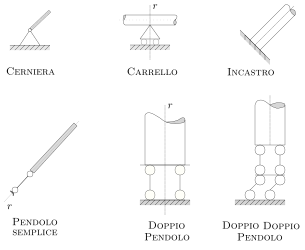
\includegraphics[width=\textwidth]{Immagini/Parte_7/Figura7_1/Figura7_1.pdf}
\caption{}
\label{figura7-1}
\end{figure}
%----------------------------------------------------------------------------------------

\noindent I vincoli esterni bidimensionali sono illustrati nella figura~\ref{figura7-1}. Il \textsc{pendolo}, come pure il \textsc{carrello}, impedisce la traslazione lungo $r$; il \textsc{doppio doppio pendolo} impedisce la rotazione. La \textsc{cerniera} impedisce entrambe le traslazioni; il \textsc{doppio pendolo} impedisce la traslazione lungo $r$ e la rotazione. L'\textsc{incastro} blocca ogni Grado di Libertà. Ne consegue che:
%----------------------------------------------------------------------------------------
%----------------------------------------------------------------------------------------
\begin{equation*}
\begin{aligned}
\textup{\textsc{pendolo}} & \\
\textup{\textsc{carrello}} & \\
\textup{\textsc{doppio doppio pendolo}} & 
\end{aligned}
\,\,\Biggr\}\,\, \textup{\textbf{Vincoli semplici}}
\end{equation*}
%----------------------------------------------------------------------------------------
%----------------------------------------------------------------------------------------
\begin{equation*}
\begin{aligned}
\textup{\textsc{cerniera}} & \\
\textup{\textsc{doppio pendolo}} & 
\end{aligned}
\,\,\Biggr\}\,\, \textup{\textbf{Vincoli doppi}}
\end{equation*}
%----------------------------------------------------------------------------------------
\noindent e infine 
%----------------------------------------------------------------------------------------
\begin{equation*}
\textup{\textsc{incastro}}\,\,\longrightarrow\,\, \textup{\textbf{Vincolo triplo}}
\end{equation*}
%----------------------------------------------------------------------------------------
\noindent Il numero di Gradi di Libertà sottratti dai suddetti vincoli resta invariato allorché essi, adoperati come vincoli interni, collegano due tronchi. La cerniera, però, \textbf{può collegare un numero qualunque di tronchi}; detto $N$ il numero di tronchi collegati, si potrebbe dimostrare che la cerniera che li collega sottrae $2(N-1)$ Gradi di Libertà. 
%----------------------------------------------------------------------------------------

\noindent È possibile tradurre in equazioni il ruolo cinematico dei vincoli e scrivere \textbf{una equazione per ogni spostamento elementare impedito}; tali equazioni sono dette di \textsc{congruenza esterna} (o di \textsc{compatibilità}); esse sono \textsc{lineari} nelle ipotesi di \textbf{spostamenti piccoli}. 
%----------------------------------------------------------------------------------------
\renewcommand{\thefigure}{7~-~2}
\begin{figure}[ht]
\centering
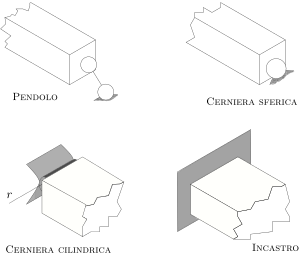
\includegraphics[width=0.75\textwidth]{Immagini/Parte_7/Figura7_2/Figura7_2.pdf}
\caption{}
\label{figura7-2}
\end{figure}
%----------------------------------------------------------------------------------------

\noindent In figura~\ref{figura7-2} sono illustrati i vincoli tridimensionali. Del pendolo già sappiamo. La \textsc{cerniera sferica} impedisce le tre traslazioni e sottrae, dunque, tre Gradi di Libertà. La \textsc{cerniera cilindrica} impedisce le tre traslazioni e due rotazioni, consentendo pertanto la sola rotazione intorno all'asse $r$; essa, dunque, sottrae cinque Gradi di Libertà. Dell'incastro già sappiamo, notando però che nello spazio esso sottrae sei Gradi di Libertà. Le cerniere sferiche e cilindriche interne, allorché collegano $N$ tronchi, sottraggono rispettivamente $3(N-1)$ e $5(N-1)$ Gradi di Libertà.
%----------------------------------------------------------------------------------------
\section{I vincoli, interpretazione statica}
%----------------------------------------------------------------------------------------
\noindent L'interpretazione statica dei vincoli è la logica conseguenza dell'interpretazione cinematica; per impedire uno spostamento lungo la retta $r$ il vincolo deve esercitare sul tronco, all'occorrenza, una \textsc{forza} avente $r$ come retta di azione; per impedire una rotazione intorno all'asse $a$ il vincolo deve esercitare sul tronco, all'occorrenza, una \textsc{coppia} il cui vettore momento sia disteso lungo $a$. Le forze ed i momenti che i vincoli esercitano sui tronchi si dicono \textsc{forze reattive} o \textsc{reazioni vincolari}. Naturalmente, \textbf{le reazioni vincolari sono le incognite nei problemi di statica}.  
%----------------------------------------------------------------------------------------

\noindent Per il \textsc{III Principio della dinamica}, il tronco esercita nel vincolo forze e/o momenti uguali ed opposti alle reazioni vincolari. 

%----------------------------------------------------------------------------------------
\renewcommand{\thefigure}{7~-~3}
\begin{figure}[ht]
\centering
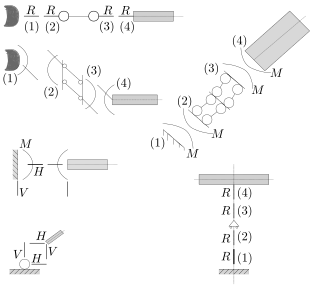
\includegraphics[width=0.72\textwidth]{Immagini/Parte_7/Figura7_3/Figura7_3.pdf}
\caption{}
\label{figura7-3}
\end{figure}
%----------------------------------------------------------------------------------------

\noindent In figura~\ref{figura7-3} è illustrato il ruolo statico dei vincoli esterni bidimensionali. Particolare attenzione merita il pendolo: le quattro forze riportate in figura hanno, ovviamente, lo stesso modulo e la stessa retta di azione, ma diversa è la loro identità fisica:
%----------------------------------------------------------------------------------------
\begin{itemize}
\item la forza indicata con $(1)$ è la forza che il suolo subisce dal pendolo;
\item la forza indicata con $(2)$ è quella che il pendolo subisce dal suolo; 
\item la forza indicata con $(3)$ è la forza che il pendolo subisce dal tronco;
\item infine, la forza indicata con $(4)$ è quella che il tronco subisce dal pendolo.
\end{itemize}
%----------------------------------------------------------------------------------------
Per il \textsc{III Principio della dinamica}, $(1)$ e $(2)$ sono uguali ed opposte e così saranno anche $(3)$ e $(4)$; si osservi, inoltre, che il pendolo è in equilibrio e non poteva essere diversamente. Nella figura~\ref{figura7-3} il pendolo \emph{tira} sul suolo e sul tronco e, a sua volta, è \emph{teso}: per questo motivo si dice che esso è un \textsc{tirante}. Si sarebbe detto che è un \textsc{puntone} se le forze avessero avuto tutte verso opposto.  È intuitivo che un tirante può realizzarsi con una sbarra rigida, ma anche con un cavo, una fune, una catena; un puntone, invece, può essere realizzato solo mediante una sbarretta rigida. Nel caso di vincoli interni colleganti due tronchi le rappresentazioni sarebbero perfettamente analoghe a quelle di figura~\ref{figura7-3}, con la sola variante di sostituire il suolo con un tronco. 
%----------------------------------------------------------------------------------------
\renewcommand{\thefigure}{7~-~4}
\begin{figure}[ht]
\centering
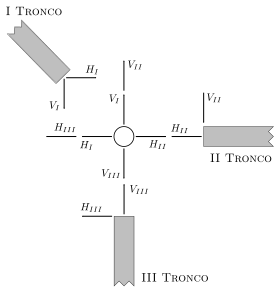
\includegraphics[width=0.65\textwidth]{Immagini/Parte_7/Figura7_4/Figura7_4.pdf}
\caption{}
\label{figura7-4}
\end{figure}
%----------------------------------------------------------------------------------------

\noindent In figura~\ref{figura7-4} è illustrato il caso di tre tronchi collegati da una cerniera. Ebbene, mentre nel caso di vincoli esterni, o interni colleganti $2$ tronchi, si riscontra una perfetta coincidenza fra il numero di Gradi di Libertà sottratti ed il numero di reazioni incognite, nel caso della cerniera in figura~\ref{figura7-4} sembra che questa coincidenza non si verifichi: sappiamo che essa sottrae $2(N-1)$ (dunque, quattro Gradi di Libertà), mentre si contano $6$ reazioni incognite. Si osservi però che, dovendo la cerniera stessa essere in equilibrio, le sei reazioni devono verificare le $2$ equazioni di equilibrio alla traslazione
%----------------------------------------------------------------------------------------
\begin{align*}
-H_I + H_{II} + H_{III} &= 0 \\ 
V_I + V_{II} - V_{III} &=0
\end{align*}
%----------------------------------------------------------------------------------------
\noindent e, pertanto, le reazioni incognite di una cerniera collegante $3$ tronchi sono, in realtà, quattro. Analogamente, per una cerniera collegante $N$ tronchi ci si convince che le reazioni incognite sono $2(N-1)$, tante quanti i Gradi di Libertà sottratti. Concludiamo questo paragrafo con la seguente 
%----------------------------------------------------------------------------------------
\begin{prop}
Ogni vincolo presenta tante reazioni incognite quanti sono i Gradi di Libertà che esso sottrae; tali reazioni agiscono nella direzione degli spostamenti impediti e, chiaramente, la reazione è un momento laddove è impedita la rotazione.
\end{prop}
%----------------------------------------------------------------------------------------
\section{Il sistema delle equazioni di equilibrio}
%----------------------------------------------------------------------------------------
Una struttura è in equilibrio \textbf{se e solo se è in equilibrio ogni suo tronco ed ogni suo vincolo}. L'equilibrio di un corpo si traduce nel fatto che le forze attive e/o reattive agenti su di esso verificano le \textsc{equazioni cardinali della statica}; in termini matematici si ha
%----------------------------------------------------------------------------------------
\begin{align*}
\underline{R} &= \underline{0} \\
\underline{M} &= \underline{0}
\end{align*}
%----------------------------------------------------------------------------------------
Queste due equazioni vettoriali sfociano in $6$ equazioni scalari nel caso tridimensionale e $3$ nel caso piano. Vale la pena sottolineare l'esatta corrispondenza fra i Gradi di Libertà posseduti da un corpo \emph{libero} ed il numero di equazioni scalari necessarie e sufficienti ad esprimere l'equilibrio; anzi, ogni equazione scalare di equilibrio viene etichettata con la stessa specificazione del corrispondente grado di libertà: \textsc{equilibrio alla traslazione lungo} $x$, $\dots$, \textsc{equilibrio alla rotazione intorno ad} $x$, $\dots$ e così via. Per quanto riguarda l'equilibrio dei vincoli, esso è, per lo più, verificato \emph{a priori}; si pensi a quanto è stato detto per il caso del pendolo. 
%----------------------------------------------------------------------------------------

\noindent Un discorso a parte va fatto per le cerniere interne, siano esse piane, sferiche o cilindriche; a proposito di essere è opportuno distinguere i seguenti casi: 
%----------------------------------------------------------------------------------------
\begin{description}
\item[\textsc{La cerniera collega} $N$ \textsc{tronchi}.] Che vi siano o meno forze direttamente concentrate su di esse, la cerniera si considera parte integrante di uno degli $N$ tronchi e, pertanto, non occorrerà alcuna equazione di equilibrio per essa, mentre le verranno attribuite $2(N-1)$, $3(N-1)$ e $5(N-1)$ incognite, a seconda che essa sia piana, sferica o cilindrica;
\item[\textsc{La cerniera collega} $1$ \textsc{solo tronco con} $2$ \textsc{o più pendoli/carrelli}.] Che vi siano o meno forze diettamente concentrate su di essa, la cerniera (piana o sferica che sia) si considera parte integrante del tronco; pertanto, non occorrerà alcuna equazione di equilibrio per essa e non le verrà attribuita alcuna incognita, essendo le incognite pari al numero di pendoli e/o carrelli che concorrono in essa;
\item[\textsc{La cerniera (piana o sferica) non tocca alcun tronco né tocca terra}.] In essa, evidentemente, concorrono solo $2$ o più pendoli e/o carrelli: in tal caso essa prende il nome di \textsc{nodo}~-~\textsc{cerniera isolato} e non viene intesa come vincolo, bensì come \textsc{punto materiale}; nessuna incognita verrà, dunque, attribuita alla cerniera; bisognerà, invece, scriverne le equazioni di equilibrio: $2$ se piana, $3$ se sferica.
\end{description}
%----------------------------------------------------------------------------------------
Ciò premesso, per scrivere le equazioni di equilibrio di una struttura, si procede come segue:
%----------------------------------------------------------------------------------------
\begin{enumerate}
\item si disegano isolate e senza vincoli tutte le \textsc{parti costituenti} della struttura. Va detto che le parti costituenti sono i \textsc{tronchi} e gli eventual \textsc{punti materiali}, tra cui le cerniere nel terzo caso precedentemente elencato;
\item in luogo dei vincoli si disegnano le rispettive \textsc{reazioni incognite}: di esse è nota la direzione, mentre sono incogniti \textbf{il modulo ed il verso}; tuttavia esse verranno disegnate con verso arbitrario; 
\item si scrivono le equazioni di equilibrio per ciascuna delle \textsc{parti costituenti}. Esse sono 
%----------------------------------------------------------------------------------------
\begin{align*}
\textup{Nello spazio}\,\,&\longrightarrow\,\,6 \forall\,\,\textup{\textsc{Tronco}} + 3 \forall\,\,\textup{\textsc{Punto materiale}} \\
\textup{Nel piano}\,\,&\longrightarrow\,\,3 \forall\,\,\textup{\textsc{Tronco}} + 2 \forall\,\,\textup{\textsc{Punto materiale}}
\end{align*}
%----------------------------------------------------------------------------------------
e le reazioni vincolari incognite saranno 
%----------------------------------------------------------------------------------------
\begin{itemize}
\item \textbf{Nello spazio} 
\begin{itemize}
\item $6\forall\,\,\textup{\textsc{Incastro}}$;
\item $5\forall\,\,\textup{\textsc{Cerniera cilindrica esterna}}$;
\item $5(N-1)\forall\,\,\textup{\textsc{Cerniera cilindrica interna}}$;
\item $3\forall\,\,\textup{\textsc{Cerniera sferica}}$;
\item $3(N-1)\forall\,\,\textup{\textsc{Cerniera sferica internica}}$;
\item $1\forall\,\,\textup{\textsc{Pendolo}}$.
\end{itemize}
\item \textbf{Nel piano}  
\begin{itemize}
\item $3\forall\,\,\textup{\textsc{Incastro}}$;
\item $2\forall\,\,\textup{\textsc{Cerniera esterna}}$;
\item $2(N-1)\forall\,\,\textup{\textsc{Cerniera interna}}$;
\item $2\forall\,\,\textup{\textsc{Doppio pendolo}}$;
\item $1\forall\,\,\textup{\textsc{Pendolo o Carrello o Doppio doppio pendolo}}$.
\end{itemize}
\end{itemize}
%----------------------------------------------------------------------------------------
\item Indicando con 
%----------------------------------------------------------------------------------------
\begin{align*}
m &= \textup{\textsc{Numero delle equazioni}} \\
n &= \textup{\textsc{Numero delle incognite}}
\end{align*}
%----------------------------------------------------------------------------------------
si ottiene un \textsc{sistema di equazioni lineari} in cui i \textsc{termini noti} sono proporzionali alle \textsc{forze attive}, i coefficienti delle incognite sono grandezze geometriche caratteristiche della struttura, le incognite sono, come già detto, le \textsc{reazioni vincolari}. Tale sistema può scriversi in termini matriciali:
%----------------------------------------------------------------------------------------
\begin{equation} \label{equazione7-1}
\begin{bmatrix}
A
\end{bmatrix}
\begin{bmatrix}
X
\end{bmatrix} 
=
\begin{bmatrix}
F
\end{bmatrix}
\tag{7.1}
\end{equation}
%----------------------------------------------------------------------------------------
con 
%----------------------------------------------------------------------------------------
\begin{align*}
\begin{bmatrix}
A
\end{bmatrix} &= \textup{\textsc{Matrice dei coefficienti}} \\
\begin{bmatrix}
X
\end{bmatrix} &= \textup{\textsc{Colonna delle incognite}} \\
\begin{bmatrix}
F
\end{bmatrix} &= \textup{\textsc{Termini noti}} 
\end{align*}
%----------------------------------------------------------------------------------------
La matrice $[ A ]$ ha ovviamente dimensioni $m\times n$; indicheremo con $r$ il suo rango. La matrice $[ X ]$ ha dimensioni $n\times 1$. La matrice che si ottiene aggiungendo ad $[ A ]$ la colonna $[ F ]$ è detta \textsc{matrice completa} 
%----------------------------------------------------------------------------------------
\begin{equation*}
\begin{bmatrix}
A_c
\end{bmatrix} 
= 
\begin{bmatrix} 
A & \vdots & F
\end{bmatrix}
\end{equation*}
%----------------------------------------------------------------------------------------
Tale matrice avrà ovviamente dimensioni $m\times(n+1)$ ed il suo rango verrà indicato con $r_c$. Risulta ovvio che
%----------------------------------------------------------------------------------------
\begin{equation*}
r\le r_c
\end{equation*}
%----------------------------------------------------------------------------------------
ed in particolare risulterà
%----------------------------------------------------------------------------------------
\begin{equation*}
\boxed{r = r_c} \,\,\Leftrightarrow\,\, \boxed{\textup{Colonna dei termini noti combinazione lineare delle colonne di } [A]}
\end{equation*}
%----------------------------------------------------------------------------------------
L'algebra lineare ci insegna che
%----------------------------------------------------------------------------------------
\begin{itemize}
\item se $r<r_c$ il sistema~\eqref{equazione7-1} è \textsc{incompatibile};
\item se $r=r_c$ il sistema~\eqref{equazione7-1} è \textsc{compatibile} ed ammette
%----------------------------------------------------------------------------------------
\begin{itemize}
\item $1$ \textsc{soluzione} se $r=n$;
\item $\infty^{n-r}$ \textsc{soluzioni} se $r<n$.
\end{itemize}
%----------------------------------------------------------------------------------------
\end{itemize}
%----------------------------------------------------------------------------------------
dire che un sistema lineare ammette $\infty^{n-r}$ soluzioni equivale a dire che le incognite non sono determinate, ma dipendono da $n-r$ parametri. Le suddette proposizioni si traducono, logicamente, nelle seguenti affermazioni a livello fisico
%----------------------------------------------------------------------------------------
\begin{itemize}
\item se $r<r_c$ \textbf{la struttura non è in equilibrio};
\item se $r=r_c$ \textbf{la struttura è in equilibrio} e le reazioni vincolari sono
%----------------------------------------------------------------------------------------
\begin{itemize}
\item \textsc{univocamente determinate} se $r=n$;
\item \textsc{indeterminate} se $r<n$ ed in tal caso esse saranno dipendenti da $n-r$ parametri.
\end{itemize}
%----------------------------------------------------------------------------------------
\end{itemize}
%----------------------------------------------------------------------------------------
\end{enumerate}
%----------------------------------------------------------------------------------------
\section{Labilità}
%----------------------------------------------------------------------------------------
\renewcommand{\thefigure}{7~-~5}
\begin{figure}[ht]
\centering
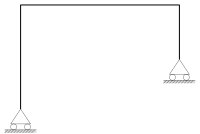
\includegraphics[width=\textwidth]{Immagini/Parte_7/Figura7_5/Figura7_5.pdf}
\caption{}
\label{figura7-5}
\end{figure}
%----------------------------------------------------------------------------------------
\noindent Una struttura si dice $l$ volte labile se essa possiede $l$ Gradi di Libertà. La struttura in figura~\ref{figura7-5}, per esempio, è $l=1$ volte labile; essa, infatti, potrebbe traslare orizzontalmente. Appare così evidente che una struttura labile \textbf{non è in equilibrio per ogni carico} ma solo per \emph{particolari} carichi, cioè per quei carichi che non ne eccitano i Gradi di Libertà. L'interpretazione statica del numero $l$ è espresa attraverso la seguente
%----------------------------------------------------------------------------------------
\begin{prop}
Una struttura si dice $l$ volte labile se i carichi attivi debbono verificare $l$ condizioni affinché essa si trovi in equilibrio.
\end{prop}
%----------------------------------------------------------------------------------------
\noindent Naturalmente, non tutte le strutture sono semplici come quella rappresentata in figura~\ref{figura7-5}; e allora bisogna trovare il modo per determinare $l$ anche nei casi più complicati.
%----------------------------------------------------------------------------------------

\noindent Ebbene, si potrebbe dimostrare, ragionando sul sistema~\eqref{equazione7-1}, che 
%----------------------------------------------------------------------------------------
\begin{equation*}
\boxed{l = m-r}
\end{equation*}
%----------------------------------------------------------------------------------------
Stabilito il valore di $l$, si pone poi il problema di individuare le $l$ condizioni di compatibilità che i carichi attivi, cioè i termini noti del sistema~\eqref{equazione7-1}, debbono verificare. Esse possono essere ottenute con le normali procedure dell'algebra lineare oppure applicando il \textbf{Principio dei Lavori Virtuali} (abbreviato in P.L.V.) dei sistemi olonomi. Talvolta è facile intuire le condizioni di compatibilità; per esempio, a proposito della figura~\ref{figura7-5}, la condizione affinché essa si trovi in equilibrio è chiaramente la seguente: deve essere nulla la componente orizzontale della risultante dei carichi attivi. Possiamo concludere questo paragrafo con la seguente, ovvia 
%----------------------------------------------------------------------------------------
\begin{prop}
Una struttura si troverà in una condizione di equilibrio per ogni sistema di carichi attivi se $l=0$. In sintesi
\begin{equation*}
\boxed{l=0\,\,\Leftrightarrow\,\, \textup{Struttura in equilibrio }\forall\textup{ carico attivo}}
\end{equation*}
\end{prop}
%----------------------------------------------------------------------------------------
\section{Indeterminazioni}
%----------------------------------------------------------------------------------------
\noindent Il numero intero non negativo 
%----------------------------------------------------------------------------------------
\begin{equation*}
\boxed{i = n-r}
\end{equation*}
%----------------------------------------------------------------------------------------
\noindent esprime, come è noto, il numero di parametri indipendenti da cui dipendono le soluzioni del sistema~\eqref{equazione7-1}, ammesso e non concesso che sia compatibile. Tali parametri si dicono \textsc{indeterminazioni} o \textsc{incognite sovrabbondanti} o ancora \textsc{incognite iperstatiche}. Il numero $i$ si presta ad una interessantissima interpretazione fisica; si consideri una struttura esente da carichi attivi e soggetta, per esempio, a \textsc{variazioni termiche}. I \textsc{termini noti} delle equazioni di equilibrio sono, pertanto, \textbf{tutti nulli}, poiché essi sono proporzionali ai carichi attivi (che abbiamo detto essere assenti) ed il sistema risulta \textsc{omogeneo}. Ebbene, se $i=0$, cioè si ha $r=n$, il sistema omogeneo ammette solo la \textbf{soluzione banale} e questo significa che le \textsc{reazioni vincolari saranno tutte nulle}. Se, invece, $i\ne 0$ e dunque $r<n$, allora il sistema ammette $\infty^i$ \textsc{soluzioni}, il che significa $\infty^i$ \textsc{possibili reazioni vincolari}. Abbiamo così dimostrato la seguente, importantissima
%----------------------------------------------------------------------------------------
\begin{prop}
Le variazioni termiche e le altre cause che non rientrino tra le forze attive \textbf{non provocheranno mai reazioni vincolari} in strutture con $i=0$. Esse, invece, \textbf{possono provocarle} in strutture con $i>0$. 
\end{prop}
%----------------------------------------------------------------------------------------
\noindent Inoltre, è ovvia anche la seguente
%----------------------------------------------------------------------------------------
\begin{prop}
Se $i=0$ le reazioni vincolari di una struttura, incognite del sistema~\eqref{equazione7-1}, risulteranno \textbf{univocamente determinate}. In termini matematici
\begin{equation*}
\boxed{i=0 \,\,\Leftrightarrow\,\, \textup{Reazioni vincolari univocamente determinate}}
\end{equation*}
\end{prop}
%----------------------------------------------------------------------------------------
\section{I quattro tipi di strutture}
%----------------------------------------------------------------------------------------
Si è potuto constatare che
%----------------------------------------------------------------------------------------
\begin{align*}
m-r &= l \\
n-r &= i
\end{align*}
%----------------------------------------------------------------------------------------
Ora, sottraendo membro a membro, si ricava quanto segue
%----------------------------------------------------------------------------------------
\begin{equation} \label{equazione7-2}
\boxed{m-n=l-i}
\tag{7.2}
\end{equation}
%----------------------------------------------------------------------------------------
Questa relazione, valida ovviamente per qualunque tipo di struttura, è utilissima allorché si voglia determinare, per una qualsiasi struttura, il valore di $l$ e di $i$; essendo $m$ ed $n$ noti \emph{a vista}, basterà conoscere $l$ per ricavare $i$ attraverso la~\eqref{equazione7-2} e viceversa. 
%----------------------------------------------------------------------------------------

\noindent La via diretta per conoscere $l$ ed $i$ passa attraverso la determinazione del rango $r$ della matrice incompleta $[ A ]$ del sistema~\eqref{equazione7-1}. Se, però, le dimensioni di $[ A ]$ sono molto grandi, la determinazione del rango può risultare particolarmente laboriosa e può dunque essere conveniente, in tal caso, valutare, con l'ausilio della cinematica, i Gradi di Libertà della struttura; poi, mediante la relazione~\eqref{equazione7-2}, essendo a questo punto noti $m$, $n$ ed $l$, si può ricavare $i$. In particolare, nel caso di strutture bidimesionali, è possibile determinare $l$ una volta individuati i \textsc{centri assoluti} e \textsc{relativi}. In ogni caso, noti $l$ ed $i$, le strutture vengono così classificate:
%----------------------------------------------------------------------------------------
\begin{enumerate}
\item \textsc{Isostatiche}: $l=0$ ed $i=0$;
\item \textsc{Iperstatiche} ($i$ \textsc{volte}): $l=0$ ed $i>0$;
\item \textsc{Labili determinate} ($l$ \textsc{volte}): $l>0$ ed $i=0$;
\item \textsc{Labili indeterminate}: $l>0$ ed $i>0$;
\end{enumerate}
%----------------------------------------------------------------------------------------
\noindent Facciamo qualche considerazione al fine di fornire una adeguata interpretazione fisica dei quattro tipi di strutture. Ecco i primi $2$ interrogativi che uno strutturista, al cospetto di una data struttura, deve porsi:
%----------------------------------------------------------------------------------------
\begin{itemize}
\item \textsc{Sarà essa in equilibrio per ogni carico attivo?}
\item \textsc{Assegnato un carico attivo ed avendo accertato che la struttura è in equilibrio, le reazioni vincolari sono univocamente determinate?}
\end{itemize}
%----------------------------------------------------------------------------------------
\begin{table}
\renewcommand\thetable{7~-~1} 
\caption{}
\label{tabella7-1}
\centering
\begin{tabular}{lcr}
\toprule
\emph{Struttura}                & \emph{Risposta al primo quesito} & \emph{Risposta al secondo quesito} \\
\midrule
\textsc{Isostatica}               & \textsc{Sì}                               & \textsc{Sì} \\
\textsc{Iperstatica}              & \textsc{Sì}                               & \textsc{No} \\
\textsc{Labile determinata}   & \textsc{No}                              & \textsc{Sì} \\
\textsc{Labile indeterminata} & \textsc{No}                              & \textsc{No} \\
\bottomrule
\end{tabular}
\end{table}
%----------------------------------------------------------------------------------------
Le risposte possibili a questi due interrogativi sono sintetizzate in tabella~\ref{tabella7-1}; le risposte suddette dovrebbero apparire ovvio alla luce del significato dei numeri $l$ ed $i$. 